\documentclass{beamer}
\usetheme{Madrid}
%\usetheme{Warsaw}

\usepackage[utf8]{inputenc}
\usepackage[T1]{fontenc}
\usepackage[russian]{babel}
\usepackage{animate}
\usepackage{amsfonts}
\usepackage{amssymb}
\usepackage{amsmath}
\usepackage{bm}
\usepackage{adjustbox}
\usepackage{diagbox}
\usepackage{csquotes}
\usepackage{caption}
\usepackage{subcaption}
\usepackage{adjustbox}
\usepackage{multirow}
\usepackage{supertabular}
\usepackage{multicol}
\usepackage{diagbox}
\usepackage{listings}
\usepackage{color}



\setbeamertemplate{caption}[numbered]
\graphicspath{{./style/}{./figures/}}

\makeatletter
\defbeamertemplate*{footline}{Dan P theme}
{
  \hbox{
  \begin{beamercolorbox}[wd = 0.5\paperwidth, ht = 2.25ex, dp = 1ex, center]{author in head/foot}
    \usebeamerfont{author in head/foot}
  \end{beamercolorbox}
	
  \begin{beamercolorbox}[wd = 0.48\paperwidth, ht = 2.25ex, dp = 1ex, right]{date in head/foot}
    \usebeamerfont{date in head/foot}\insertshortdate{}\hspace*{2em}
		
\insertframenumber{} / \inserttotalframenumber\hspace*{2ex} 
  \end{beamercolorbox}}
	
  \vskip0pt
}
\makeatother


\renewcommand{\phi}{\varphi}

\renewcommand{\kappa}{\varkappa}

%\usecolortheme{default}
%\usecolortheme{seahorse}
%\usecolortheme{dolphin} % Синий цвет
%\usecolortheme{beetle}  % Темно-зеленый цвет
%\usecolortheme{crane}   % Оранжевый цвет
%\usecolortheme{rose}    % Розовый цвет
%\usecolortheme{seagull} % Серый цвет

%\setbeamercolor{background canvas}{bg=blue!10} % Задний фон слайдов
%\setbeamercolor{title}{fg=white, bg=blue}      % Заголовки слайдов
%\setbeamercolor{frametitle}{fg=white, bg=orange} % Фон и текст заголовка фрейма
%\setbeamercolor{block title}{fg=white, bg=orange} % Цвет блоков
%\setbeamercolor{block body}{bg=red!10}         % Тело блоков
%\setbeamercolor{author in head/foot}{bg=gray!30, fg=black} % Нижний колонтитул
%\setbeamercolor{date in head/foot}{bg=gray!30, fg=black}   % Нижний колонтитул

%\usepackage{xcolor}

% Определение собственных цветов
%\definecolor{myblue}{RGB}{0, 123, 255}
%\definecolor{mygray}{RGB}{45, 45, 45}

% Применение цветов
%\setbeamercolor{background canvas}{bg=myblue!10}
%\setbeamercolor{title}{fg=mygray, bg=myblue!30}

\definecolor{dkgreen}{rgb}{0,0.6,0}
\definecolor{gray}{rgb}{0.5,0.5,0.5}
\definecolor{mauve}{rgb}{0.58,0,0.82}

\lstset{frame=tb,
	inputencoding=utf8,
	basicstyle=\ttfamily,
	extendedchars=\true,
	showspaces=\false,
	showstringspaces=\false,
	language=Python,
	aboveskip=3mm,
	belowskip=3mm,
	showstringspaces=false,
	columns=flexible,
	basicstyle={\small},
	numbers=left,
	numberstyle=\tiny\color{gray},
	%keywordstyle=\color{red},
	%commentstyle=\color{dkgreen},
	%stringstyle=\color{mauve},
	keywordstyle=\color{black},
	commentstyle=\color{black},
	stringstyle=\color{black},
	breaklines=true,
	breakatwhitespace=true,
	tabsize=3
}

\usepackage{progressbar}

\setbeamertemplate{footline}{
	\hbox{
		\begin{beamercolorbox}[wd=\paperwidth,ht=2.25ex,dp=1ex,right]{date in head/foot}
			% Условие: меняем стиль нумерации после 2-го слайда
			\ifnum\insertframenumber<19
			 \insertframenumber{} / 18
			\else
			\insertframenumber{}
			\fi
			\hspace*{2ex}
		\end{beamercolorbox}
	}
	\vskip0pt
}

\usepackage{graphicx}
\usepackage{tikz}

\setbeamertemplate{background}{
	\ifnum\insertframenumber=1 % Проверяем номер слайда
	
\includegraphics[width=\paperwidth,height=1.05\paperheight]{fon7}
	\fi
}




\begin{document}


\title{Применение нейронных сетей\\для улучшения решения уравнения переноса}
\author{Выполнил: Климов О.\,Д., ФН2--71Б \\ под руководством д. ф.-м. н. Галанина М.\,П.}
%\date{\today}
\date{}


\begin{frame}
\begin{figure}[!hp]
	
\includegraphics[width=0.14\textwidth]{logo/logo1}
	
\includegraphics[width=0.15\textwidth]{logo/logo2}
\end{figure}
\titlepage
\end{frame}





\section{Постановка задачи}
\begin{frame}
\frametitle{Постановка задачи}
\begin{block}{Формулировка}
\begin{enumerate}
	\item Необходимо для одномерного уравнения переноса реализовать алгоритм улучшения решения на основе искусственных нейронных сетей.
	\item  Протестировать работу программы на системе из 5 тестов (рис.\ref{primer_nabor}):\\ левый и правый треугольники, прямоугольник, косинус, зуб. \hyperlink{pril1}{\beamergotobutton{Приложение 1}}
	 
\end{enumerate}
\end{block}

\begin{figure}[!hp]
	\centering
	\begin{tabular}{ccccc@{\hspace{0.5cm}}ccccc}
		\begin{subfigure}[t]{0.17\textwidth}
			\centering
			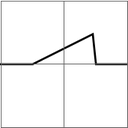
\includegraphics[width=\textwidth]{1}
			\caption{Тест 1}
			\label{test1}
		\end{subfigure} &
		\begin{subfigure}[t]{0.17\textwidth}
			\centering
			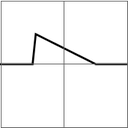
\includegraphics[width=\textwidth]{2}
			\caption{Тест 2}
			\label{test2}
		\end{subfigure} & 
		\begin{subfigure}[t]{0.17\textwidth}
			\centering
			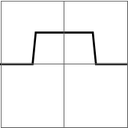
\includegraphics[width=\textwidth]{3}
			\caption{Тест 3}
			\label{test3}
		\end{subfigure} &
		\begin{subfigure}[t]{0.17\textwidth}
			\centering
			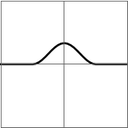
\includegraphics[width=\textwidth]{4}
			\caption{Тест 4}
			\label{test4}
		\end{subfigure} &
		\begin{subfigure}[t]{0.17\textwidth}
			\centering
			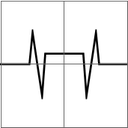
\includegraphics[width=\textwidth]{5}
			\caption{Тест 5}
			\label{test5}
		\end{subfigure} 
	\end{tabular}
	\caption{Система тестов}
	\label{primer_nabor}
\end{figure}
\end{frame}





\section{Уравнение переноса}

\frametitle{Уравнение переноса}
\begin{frame}
\frametitle{Уравнение переноса}
	\begin{block}{Задача Коши для уравнения переноса}
		\begin{equation}
			\begin{cases}
				\dfrac{\partial u}{\partial t} + a\dfrac{\partial u}{\partial x} = 0, \\
				u(x, 0) = u_0(x),
			\end{cases} 
			\text{где } \quad a = const > 0, \quad t \in (0, T) .
		\end{equation}
		
		Решение имеет вид $u = u_0(x-at)$ и заключается в сносе неизменного профиля по характеристикам. Численные схемы имеют ряд проблем.
	\end{block}
	
	\vspace{-0.5em}
	\begin{figure}[!h]
		\centering
		\begin{subfigure}[t]{0.44\textwidth}
			\centering
			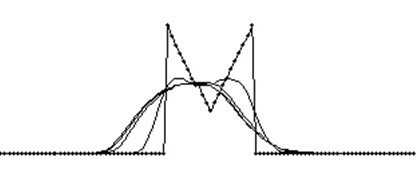
\includegraphics[width=\textwidth]{prim1}
			\caption{Пример схемы с диссипацией}
		\end{subfigure}
		\quad\quad\quad
		\begin{subfigure}[t]{0.44\textwidth}
			\centering
			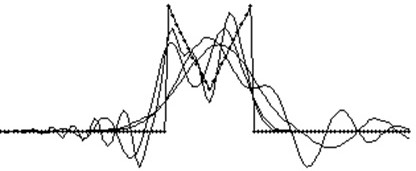
\includegraphics[width=\textwidth]{prim2}
			\caption{Пример схемы с дисперсией}
		\end{subfigure}
		\vspace{-1em}
		\caption{Пример точного (буква М) и численного решения уравнения переноса при некоторых различных числах Куранта. Иллюстрации взяты из \cite[c.416]{1}} .
	\end{figure}
\end{frame}
	
	
\section{Технологии нейронных сетей}

\begin{frame}
	\frametitle{Технологии нейронных сетей}
	\begin{block}{Понятие нейронной сети}
	 \textbf{Нейронная сеть} --- это модель основанная на принципе организации биологических нейронных сетей. Ее можно интерпретировать совершенно по-разному.
	\end{block}
	\begin{block}{Нейрон}
	\textbf{Нейрон} --- единица обработки информации в нейронной сети, который можно представить функцией \cite[c.28]{7}, \hyperlink{pril2}{\beamergotobutton{Приложение 2}}
	\begin{equation}
		y_k = \phi(u_k + b_k), \quad u_k = \sum_{j = 1}^{m} w_{kj}x_j 
		\label{1}
	\end{equation}
	где $x_1, x_2, \dots, x_m$ --- входные сигналы, \\
	$w_{k1}, w_{k2}, \dots, w_{km}$ --- веса связей нейрона $k$, \\
	$u_k $ --- линейная комбинация входных воздействий,
	$b_k$ --- порог,\\
	$ \phi $ --- функция активации,
	$ y_k $ --- выходной сигнал.
	\end{block}
\end{frame}

\begin{frame}
	\frametitle{Технологии нейронных сетей}
	\begin{block}{Функции активации}
		\begin{itemize}
			\item $\phi(x) =  \dfrac{1}{1+\exp^{-x}} \quad\textbf{--- Сигмоида} $
			\item $\phi(x) =  \max(0, x)  \quad\textbf{--- ReLU}$
		\end{itemize} 
	\end{block}
	\begin{block}{Структура сети}
		В нейронной сети нейроны упорядочено располагаются по слоям и связываются между собой направленными связями. Каждый нейрон принимает входные сигналы от нейронов предыдущего слоя, преобразует их с помощью весов и функции активации и передает результат на следующий слой. 
	\end{block}
	\begin{itemize}
		\item \textbf{Входной слой} --- принимает $x = (x_1, x_2, \dots, x_m)$
		\item \textbf{Скрытые слои} --- выполняют основную обработку информации
		\item \textbf{Выходной слой} --- представляет результат $y = (y_1, y_2, \dots, x_n)$
	\end{itemize} 
\end{frame}

\begin{frame}
	\frametitle{Технологии нейронных сетей}
	\begin{block}{Обучение сети}
		\textbf{Обучением нейронной сети} называется процесс настройки весов $w_{ij}$ таким образом, минимизировать ошибку между результатом сети и целевым значением на обучающем наборе данных. \cite[c.85]{2}\\
		Вводят функцию потерь $L(y_{pred},y_{true}) = \frac{1}{n} \sum_{i=1}^{n} (y_{pred, i} - y_{true, i})^2$
	\end{block}
	\begin{block}{Алгоритм метода обратного распространения ошибки}
		\begin{enumerate}
			\item \textbf{Прямой ход:} \\
			 для входных данных $x$ вычисляется результат $y$
			\item \textbf{Обратный ход:} вычисляется\\
			$\delta_k = \frac{\partial L}{\partial y_k} \cdot \phi'(u_k)$ --- ошибка на выходном слое \\
			$\delta_j = \sum_{k=1}^{n} \delta_k w_{kj} \cdot \phi'(u_j)$ --- ошибка на скрытых слоях
			
			\item \textbf{Обновление параметров:} 
			$w_{kj} := w_{kj} - \eta \cdot \frac{\partial L}{\partial w_{kj}},$ \\ где $\frac{\partial L}{\partial w_{kj}} = \delta_k \cdot x_j$,\quad $\eta$ --- скорость обучения 
		\end{enumerate}
	\end{block}
	
	
\end{frame}

\begin{frame}
	\frametitle{Технологии нейронных сетей}
	\begin{block}{Сверточная нейронная сеть}
		\textbf{Сверточная нейронная сеть} --- особый тип сетей, который характеризуется наличием операций свертки и пуллинга. 
	\end{block}
	\begin{block}{Свертка и пуллинг \hyperlink{pril3}{\beamergotobutton{Приложение 3}}}
	\textbf{Операция свертки} для матрицы \(x\) и ядра свертки \(w\) с размером \(h \times h\) определяется следующим образом:
	\vspace{-0.5em}
	\[ y_{ij} = \sum_{m=0}^{h-1} \sum_{n=0}^{h-1} x_{i+m, j+n} \cdot w_{mn}. \]
	\vspace{-1em}
	
	Для сохранения исходной размерности добавляют нулевой \textbf{паддинг} --- обрамление изображение нулями.  Без паддинга размер уменьшается на $(h - 1)$ пикс. по каждому измерению. 
	
	Слои \textbf{пуллинга} (подвыборки) производят функцию уменьшения размерности данных при сохранении признаков.
	\end{block}
\end{frame}



\section{Реализация алгоритма}

\begin{frame}
	\frametitle{Реализация алгоритма}
	\vspace{-0.5em}
	\begin{block}{Методика подготовки наборов данных}
		\begin{itemize}
			\item Пары изображений "<шумное-идеальное"> созданы с помощью Wolfram Mathematica. 
			\item $128x128$ px --- размер изображения, канал ч/б
			\item $3$ теста --- левый и правый треугольник, прямоугольник, тесты 4, 5 оставлены для тестирования
			\item 2 обучающих набора данных: однородные и неоднородные фигуры соответственно. Набор №1 --- 500 пар,  набор №2 --- 2000 пар
		\end{itemize}
	\end{block}
	\begin{block}{Способ реализации программы}
		\begin{itemize}
			\item Язык программирования Python, фреймворк TensorFlow (TF)
			\item Использование функций создания моделей и их обучения из TF
			\item Собственная реализация функций работы с наборами данных, их визуализации и расчета оценок
		\item Использование графического процессора для расчетов 
		\end{itemize}
	\end{block}
\end{frame}

\begin{frame}
	%\frametitle{Реализация алгоритма}
		\begin{figure}[!hp]
			\centering
			\begin{tabular}{cc@{\hspace{1cm}}cc}
				% Первая строка изображений
				\begin{subfigure}[t]{0.2\textwidth}
					\centering
					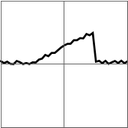
\includegraphics[width=\textwidth]{nabor1_1}
				\end{subfigure} &
				\begin{subfigure}[t]{0.2\textwidth}
					\centering
					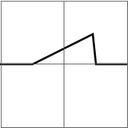
\includegraphics[width=\textwidth]{nabor1_2}
				\end{subfigure} &
				\begin{subfigure}[t]{0.2\textwidth}
					\centering
					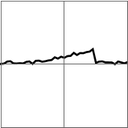
\includegraphics[width=\textwidth]{nabor2_1}
				\end{subfigure} &
				\begin{subfigure}[t]{0.2\textwidth}
					\centering
					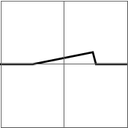
\includegraphics[width=\textwidth]{nabor2_2}
				\end{subfigure} \\
				\multicolumn{2}{c}{\small (a) Тест 1 из набора №1} &
				\multicolumn{2}{c}{\small (d) Тест 1 из набора №2} \\
				
				% Вторая строка изображений
				\begin{subfigure}[t]{0.2\textwidth}
					\centering
					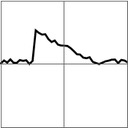
\includegraphics[width=\textwidth]{nabor1_3}
				\end{subfigure} &
				\begin{subfigure}[t]{0.2\textwidth}
					\centering
					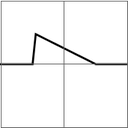
\includegraphics[width=\textwidth]{nabor1_4}
				\end{subfigure} &
				\begin{subfigure}[t]{0.2\textwidth}
					\centering
					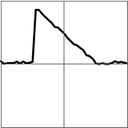
\includegraphics[width=\textwidth]{nabor2_3}
				\end{subfigure} &
				\begin{subfigure}[t]{0.2\textwidth}
					\centering
					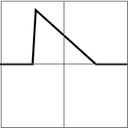
\includegraphics[width=\textwidth]{nabor2_4}
				\end{subfigure} \\
				\multicolumn{2}{c}{\small (b) Тест 2 из набора №1} &
				\multicolumn{2}{c}{\small (e) Тест 2 из набора №2} \\
				
				% Третья строка изображений
				\begin{subfigure}[t]{0.2\textwidth}
					\centering
					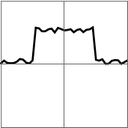
\includegraphics[width=\textwidth]{nabor1_5}
				\end{subfigure} &
				\begin{subfigure}[t]{0.2\textwidth}
					\centering
					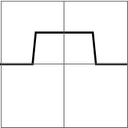
\includegraphics[width=\textwidth]{nabor1_6}
				\end{subfigure} &
				\begin{subfigure}[t]{0.2\textwidth}
					\centering
					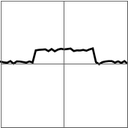
\includegraphics[width=\textwidth]{nabor2_5}
				\end{subfigure} &
				\begin{subfigure}[t]{0.2\textwidth}
					\centering
					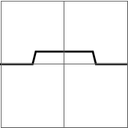
\includegraphics[width=\textwidth]{nabor2_6}
				\end{subfigure} \\
				\multicolumn{2}{c}{\small (c) Тест 3 из набора №1} &
				\multicolumn{2}{c}{\small (f) Тест 3 из набора №2} \\
			\end{tabular}
			\caption{Примеры пар изображений из наборов данных}
			\label{fig:grid_example}
		\end{figure}
\end{frame}

\begin{frame}
	\frametitle{Реализация алгоритма}
	\begin{block}{Архитектура модели \hyperlink{pril4}{\beamergotobutton{Приложение 4}}}
		%Архитектура сети состоит из нескольких сверточных слоев и механизмов декодирования для восстановления изображения:
		
		\begin{itemize}
			\item \textbf{Входной слой:} Принимает изображения размером $128 \times 128$ с одним каналом (градации серого). 
			
			\item \textbf{Сверточные слои:} Используются 4 последовательные свертки с ядром размером $3 \times 3$. Каждая свертка сопровождается функцией активации \texttt{ReLU}.
			
			\item \textbf{Уменьшение размерности (MaxPooling):} После сверточных слоев применяется слой пулинга с блоком $2 \times 2$.
			\item \textbf{Декодирующие слои (UpSampling):} На этапе восстановления разрешения используются транспонированные свертки с ядром $3 \times 3$ и операцией увеличения размера (UpSampling) для восстановления изображения до исходного размера.
			
			\item \textbf{Выходной слой:} Завершающий слой с функцией активации \texttt{sigmoid}, который возвращает выходное изображение.
		\end{itemize}
	\end{block}
\end{frame}




\section{Результаты}

\begin{frame}
	\vspace{-0.75em}
	\begin{block}{Расчет оценок}
		$\kappa = L_{in} - L_{out}$, $\psi = L_{in} / L_{out}$, где $L_{in} = L(x, y_{true})$, $L_{out} = L(y_{pred}, y_{true})$
	 \end{block}
	 
	\vspace{-0.5em}
	\frametitle{Результаты для набора №1}
	%\vspace{-1em}
	\begin{figure}[!hp]
		\centering
		% Первая строка
		\begin{subfigure}{\textwidth}
			\centering
			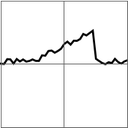
\includegraphics[width=0.22\textwidth]{res_n1_1}
			\hfill
			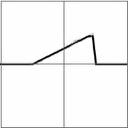
\includegraphics[width=0.22\textwidth]{res_n1_2}
			\hfill
			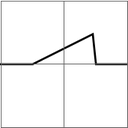
\includegraphics[width=0.22\textwidth]{1}
			\caption*{\small (a) Тест 1 для набора №1: $L_{in} = 0.0198, 
				L_{out} = 0.0003, 
				\kappa = 0.0194,
				\psi = 60.07
				$}
		\end{subfigure}
		\vspace{-1.2em}
		% Вторая строка
		\begin{subfigure}{\textwidth}
			\centering
			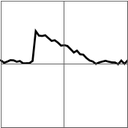
\includegraphics[width=0.22\textwidth]{res_n1_3}
			\hfill
			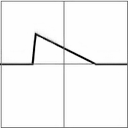
\includegraphics[width=0.22\textwidth]{res_n1_4}
			\hfill
			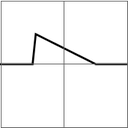
\includegraphics[width=0.22\textwidth]{2}
			\caption*{\small (b) Тест 2 для набора №1: $L_{in} = 0.0205, 
				L_{out} = 0.0001,
				\kappa = 0.0204,
				\psi = 254.75
				$}
		\end{subfigure}
	\end{figure}
\end{frame}

\begin{frame}
		\frametitle{Результаты для набора №1}
		\vspace{-1em}
		\begin{figure}[!hp]
			\centering
			% Первая строка
			\begin{subfigure}{\textwidth}
				\centering
				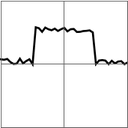
\includegraphics[width=0.27\textwidth]{res_n1_5}
				\hfill
				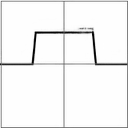
\includegraphics[width=0.27\textwidth]{res_n1_6}
				\hfill
				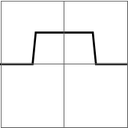
\includegraphics[width=0.27\textwidth]{3}
				\caption*{\small (c) Тест 3 для набора №1: $L_{in} = 0.0195,
					L_{out} = 0.0001,
					\kappa = 0.0194,
					\psi = 220.01$}
			\end{subfigure}
			\vspace{-1.2em}
			% Вторая строка
			\begin{subfigure}{\textwidth}
				\centering
				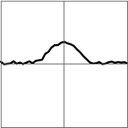
\includegraphics[width=0.27\textwidth]{res_n1_7}
				\hfill
				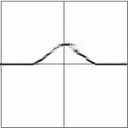
\includegraphics[width=0.27\textwidth]{res_n1_8}
				\hfill
				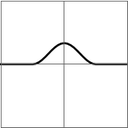
\includegraphics[width=0.27\textwidth]{4}
				\caption*{\small (d) Тест 4 для набора №1: $L_{in} = 0.0218,
					L_{out} = 0.0043,
					\kappa = 0.017,
					\psi = 5.06
					$}
			\end{subfigure}
		\end{figure}
\end{frame}

\begin{frame}
	\frametitle{Результаты для набора №1 \hyperlink{pril5}{\beamergotobutton{Дополнительные результаты в Приложение 5}}}
	\vspace{-0.5em}
	\begin{figure}[!hp]
		\centering
		% Первая строка
	\begin{subfigure}{\textwidth}
	\centering
	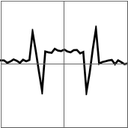
\includegraphics[width=0.27\textwidth]{res_n1_9}
	\hfill
	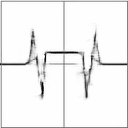
\includegraphics[width=0.27\textwidth]{res_n1_10}
	\hfill
	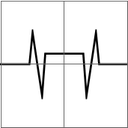
\includegraphics[width=0.27\textwidth]{5}
	\caption*{\small (e) Тест 5 для набора №1: $L_{in} = 0.0185,
		L_{out} = 0.0108, 
		\kappa = 0.0076,
		\psi = 1.71$}
	\end{subfigure}
	\vspace{-2em}
	\caption{Результаты для набора №1 ("<входное-выходное-целевое"> изобр.)}
\end{figure}
\vspace{-1.5em}
\begin{table}[!ht]
	\centering
	\caption{Результаты тестирования алгоритма для набора данных №1 }
	\vspace{-0.75em}
	\large
	\begin{tabular}{|c|c|c|c|c|}
		\hline
		\textbf{Тип теста} & \(\mathbf{L_{in}}\) & \(\mathbf{L_{out}}\) & \(\mathbf{\kappa}\) & \(\mathbf{\psi}\) \\ \hline
		Тест 1 & 0.0198 & 0.0003 & 0.0194 & 60.07 \\ \hline
		Тест 2 & 0.0205 & 0.0001 & 0.0204 & 254.75 \\ \hline
		Тест 3 & 0.0195 & 0.0001 & 0.0194 & 220.01 \\ \hline
		Тест 4 & 0.0218 & 0.0043 & 0.0170 & 5.06 \\ \hline
		Тест 5 & 0.0185 & 0.0108 & 0.0076 & 1.71 \\ \hline
	\end{tabular}
	\label{tab:results}
\end{table}
\end{frame}



\begin{frame}
	\frametitle{Результаты для набора №2}
	\vspace{-1em}
	\begin{figure}[!hp]
		\centering
		% Первая строка
		\begin{subfigure}{\textwidth}
			\centering
			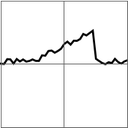
\includegraphics[width=0.27\textwidth]{res_n1_1}
			\hfill
			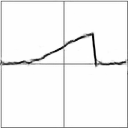
\includegraphics[width=0.27\textwidth]{res_n2_2}
			\hfill
			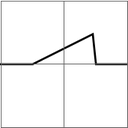
\includegraphics[width=0.27\textwidth]{1}
			\caption*{\small (a) Тест 1 для набора №1: 
				$L_{in} = 0.0198,
				L_{out} = 0.0107, 
				\kappa = 0.0091,
				\psi = 1.84
				$}
		\end{subfigure}
		% Вторая строка
		\vspace{-1em}
		\begin{subfigure}{\textwidth}
			\centering
			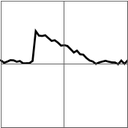
\includegraphics[width=0.27\textwidth]{res_n1_3}
			\hfill
			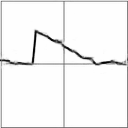
\includegraphics[width=0.27\textwidth]{res_n2_4}
			\hfill
			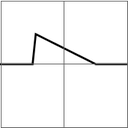
\includegraphics[width=0.27\textwidth]{2}
			\caption*{\small (b) Тест 2 для набора №1:
				$L_{in} = 0.0205,
				L_{out} = 0.0118,
				\kappa = 0.0087,
				\psi = 1.73
				$}
		\end{subfigure}
	\end{figure}
\end{frame}

\begin{frame}
	\frametitle{Результаты для набора №2}
	\vspace{-2em}
	\begin{figure}[!hp]
		\centering
			% Третья строка
		\vspace{1em}
		\begin{subfigure}{\textwidth}
			\centering
			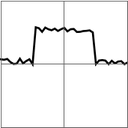
\includegraphics[width=0.27\textwidth]{res_n1_5}
			\hfill
			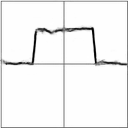
\includegraphics[width=0.27\textwidth]{res_n2_6}
			\hfill
			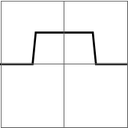
\includegraphics[width=0.27\textwidth]{3}
			\caption*{\small (c) Тест 3 для набора №1: $L_{in} = 0.0195, L_{out} = 0.0109, \kappa = 0.0086, \psi = 1.78$}
		\end{subfigure}
		% Четвертая строка
			\vspace{-1em}
		\begin{subfigure}{\textwidth}
			\centering
			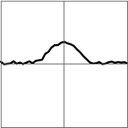
\includegraphics[width=0.27\textwidth]{res_n1_7}
			\hfill
			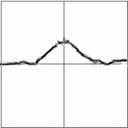
\includegraphics[width=0.27\textwidth]{res_n2_8}
			\hfill
			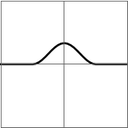
\includegraphics[width=0.27\textwidth]{4}
			\caption*{\small (d) Тест 4 для набора №2: $L_{in} = 0.0218, L_{out} = 0.0105, \kappa = 0.0113, \psi = 2.08$}
		\end{subfigure}
	\end{figure}
\end{frame}

\begin{frame}
	\frametitle{Результаты для набора №2 \hyperlink{pril6}{\beamergotobutton{Дополнительные результаты в Приложение 6}}}
	\vspace{-0.5em}
	\begin{figure}[!hp]
		\centering
		\begin{subfigure}{\textwidth}
		\centering
		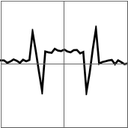
\includegraphics[width=0.27\textwidth]{res_n1_9}
		\hfill
		\includegraphics[width=0.27\textwidth]{res_n2_10}
		\hfill
		\includegraphics[width=0.27\textwidth]{5}
		\caption*{\small (d) Тест 5 для набора №2: $L_{in} = 0.0185, L_{out} = 0.0130, \kappa = 0.0055, \psi = 1.41$}
	\end{subfigure}
	\vspace{-2em}
	\caption{Результаты для набора №2 ("<входное-выходное-целевое"> изобр.)}
\end{figure}
\vspace{-1.5em}
\begin{table}[!ht]
\centering
\caption{Результаты тестирования алгоритма для набора данных №2 }
\vspace{-0.75em}
	\large
	\begin{tabular}{|c|c|c|c|c|}
		\hline
		\textbf{Номер теста} & \(\mathbf{L_{in}}\) & \(\mathbf{L_{out}}\) & \(\mathbf{\kappa}\) & \(\mathbf{\psi}\) \\ \hline
		Тест 1 & 0.0198 & 0.0107 & 0.0091 & 1.84 \\ \hline
		Тест 2 & 0.0205 & 0.0118 & 0.0087 & 1.73 \\ \hline
		Тест 3 & 0.0195 & 0.0109 & 0.0086 & 1.78 \\ \hline
		Тест 4 & 0.0218 & 0.0105 & 0.0113 & 2.08 \\ \hline
		Тест 5 & 0.0185 & 0.0130 & 0.0055 & 1.41 \\ \hline
	\end{tabular}
	\label{tab:results2}
\end{table}
\end{frame}




\section{Заключение}
\begin{frame}
	\frametitle{Заключение}
	\begin{block}{Перспективы задачи}
		\begin{itemize} 
			\item Дальнейшее исследование оптимизации модели
			\item Обучать модели на реальных данных, основанных на численных решениях определенных разностных схем
			\item Рассмотреть другие архитектуры моделей или, например, подход \textbf{обучения без учителя}
		\end{itemize} 
	\end{block}
	\begin{block}{Итог}
		\begin{itemize}
			\item Рассмотрены технологии нейронных сетей
			\item Разработан алгоритм улучшения решения уравнения переноса
			\item Созданы 2 набора данных
			\item Реализована программа и протестирована на системе тестов исходной задачи с примерами результатов
		\end{itemize}
	\end{block}
\end{frame}




\begin{frame}
	\frametitle{Список литературы}
	\vspace{-0.5em}
	\small
	\begin{thebibliography}{10}
		
	\bibitem{1} Галанин М.П., Савенков Е.Б. Методы численного анализа математических моделей. — М.: Изд-во МГТУ им. Н.Э. Баумана, 2018. — 592 с. --- ISBN 978-5-7038-4796-1
	
	\bibitem{7}  Хайкин С. Нейронные сети: полный курс.:,пер. с англ., 2-е изд. — М.: Издательский дом «Вильямс», 2006. — 1104 с. — ISBN 5-8459-0890-6.
	
	\bibitem{2} Rashid T. Make Your Own Neural Network. — CreateSpace Independent Publishing Platform, 1st edition, 2016. — SAND96-0583.
	
	\bibitem{3} Николенко С., Кадурин А., Архангельская Е. Глубокое обучение. — СПб.: Питер, 2022. — 476 с. — ISBN 978-5-4461-1537-2.
	
	\bibitem{9} Шолле Ф. Глубокое обучение на Python. — СПб.: Питер, 2018. — 400 с. — ISBN 978-5-4461-0770-4.
	
	\vspace{-0.1em}
	\bibitem{10} Гафаров Ф.М., Галимянов А.Ф. Искусственные нейронные сети и приложения: учебное пособие. — Казань: Изд-во Казан. ун-та, 2018. — 121 с.
	
	\vspace{-0.1em}
	\bibitem{6} Машинное обучение и TensorFlow. — СПб.: Питер, 2019. — 336 с. — ISBN 978-5-4461-0826-8.
	
	\end{thebibliography}
\end{frame}






\appendix
%\addtocounter{framenumber}{-8} % Уменьшаем счётчик на количество слайдов приложени
%\setcounter{framenumber}{0} % Сбросить счётчик слайдов
%\setbeamertemplate{footline}{} % Убираем футер для приложения
%\appendix

\begin{frame}
	\label{pril1}
	\frametitle{Приложение 1: Начальные условия для системы тестов}
	\begin{equation*}
		(\ref{test1}):  u_0(x) = \frac{x-l_1}{l_2-l_1} \quad \text{--- левый треугольник,}
	\end{equation*}
	\begin{equation*}
		(\ref{test2}): u_0(x) = \frac{l_2-x}{l_2-l_1} \quad \text{--- правый треугольник,}
	\end{equation*}
	\begin{equation*}
		(\ref{test3}): u_0(x) = \frac{2}{3} \quad \text{--- прямоугольник}
	\end{equation*}
	\begin{equation*}
		(\ref{test4}): u_0(x) = \frac{1}{3} (1 - \cos(\frac{2 \pi (x - l_1)}{l_2 - l_1})) \quad \text{--- косинус}
	\end{equation*}
	\begin{equation*}
		(\ref{test5}): u_0(x) =
		\begin{cases} 
			-\frac{2}{3} (l_{11} - l_1) (x - l_1) + 1, & l_1 \leq x < l_{11},\\
			\frac{1}{3}, & l_{11} \leq x \leq l_{22}, \\
			\frac{2}{3} (l_2 - l_{22}) (x - l_2) + 1, & l_{22}, < x \leq l_2
		\end{cases}
		\quad \text{--- зуб,}
	\end{equation*}

\end{frame}

\begin{frame}
	\label{pril2}
	\frametitle{Приложение 2: Преобразование порога для модели нейрона}
	Использование порога $b_k$ обеспечивает эффект аффинного преобразования выхода линейного сумматора $u_k$. В частности, в зависимости от того, какое значение принимает порог,  положительное или отрицательное, можно двигать значения выхода нейрона. Обозначим $w_{k0} = b_k$ и преобразуем модель к следующему виду
	\begin{equation}
		y_k = \phi(v_k), \quad v_k = \sum_{j = 0}^{m} w_{kj}x_j 
		\label{2}
	\end{equation}
	
	\vspace{-0.5em}
	Таким образом, в выражении \eqref{2} добавился новый синапс. Его входной сигнал и вес соответственно равны
	\begin{equation*}
		x_0 = +1, \quad w_{k0} = b_k.
	\end{equation*}
	Это позволило трансформировать модель нейрона к виду, при котором добавляется новый входной сигнал фиксированной величины $+1$, а также появляется новый синаптический вес, равный пороговому значению $b_k$. 
\end{frame}

\begin{frame}
	\label{pril3}
	\frametitle{Приложение 3: Визуализация сверточной нейронной сети}
	\begin{figure}[!hp]
		\centering
		\includegraphics[width=0.9\textwidth]{conv}
	\end{figure}
	\[ y_{ij} = \sum_{m=0}^{h-1} \sum_{n=0}^{h-1} x_{i+m, j+n} \cdot w_{mn} \quad \text{--- Cвертка} \]
	\[ x_{i+m, j+n} = \sum_{m'=0}^{h-1} \sum_{n'=0}^{h-1} y_{i+m', j+n'} \cdot w_{m'n'} \quad \text{ --- Транспонированная свертка} \]
\end{frame}

\begin{frame}
	\label{pril4}
	\vspace{-0.5em}
	\frametitle{Приложение 4 ч1: Программа модели сети}
	\begin{figure}[!hp]
		\centering
		\vspace{-0.1em}
		\begin{subfigure}[t]{0.45\textwidth}
			\centering
			\includegraphics[width=\textwidth]{model_diagram1}
		\end{subfigure}
		\begin{subfigure}[t]{0.45\textwidth}
			\centering
			\includegraphics[width=\textwidth]{model_diagram2}
		\end{subfigure} 
	\vspace{-0.6em}
	\caption{Диаграмма модели}
	\label{model_diagram}
	\end{figure}
\end{frame}

\begin{frame}
	\frametitle{Приложение 4 ч2: Программа модели сети}
	\centering
	\adjustbox{scale=0.7}{
		\lstinputlisting[caption={Модель нейронной сети c использованием TF}, inputencoding=utf8]{code/Model.py}
	}
\end{frame}

\begin{frame}
	\frametitle{Приложение 4 ч3: Программа модели сети}
	\begin{block}{Особенности реализации}
	\begin{itemize}
		\item Модель представляет собой сверточный автокодировщик
		\item Модель имеет 296.217 параметров
		\item Набор предварительно перемешивается с целью избежать корреляций между последовательными данными
		\item В процессе обучения в каждой эпохе вычисляется наименьшее значение потерь на валидационной выборке и, в случае увеличения ее значения, сохраняется предыдущая модель
		\item Использована опция предзагрузки данных, где для следующей эпохи обучения данные параллельно загружаются, пока обрабатывается текущая эпоха, причем учитывая специфику системы и загрузку процессора.
		\item Для набора №1 оптимальным выбрано 100 эпох обучения, для набора №2 около 70
	\end{itemize}
	\end{block}
\end{frame}

\begin{frame}
	\label{pril5}
	\frametitle{Приложение 5 ч.1: Доп. результаты, набор №1}
\begin{table}[!ht]
	\centering
	\caption{Результаты модели, обученной на наборе №1, при тестировании на валидационном наборе №2 (не входил в обучающую выборку)}
	\vspace{-0.75em}
	\large
	\begin{tabular}{|c|c|c|c|c|}
		\hline
		\textbf{Номер теста} & \(\mathbf{L_{in}}\) & \(\mathbf{L_{out}}\) & \(\mathbf{\kappa}\) & \(\mathbf{\psi}\) \\ \hline
		Тест 1 & 0.0113 & 0.0063 & 0.0050 & 1.79 \\ \hline
		Тест 2 & 0.0093 & 0.0071 & 0.0022 & 1.31 \\ \hline
		Тест 3 & 0.0104 & 0.0096 & 0.0008 & 1.08 \\ \hline
		Тест 4 & 0.0129 & 0.0052 & 0.0076 & 2.46 \\ \hline
		Тест 5 & 0.0095 & 0.0050 & 0.0045 & 1.90 \\ \hline
	\end{tabular}
	\label{tab:results2}
	\end{table}
	\begin{figure}[!hp]
		\centering
		\begin{tabular}{ccccc@{\hspace{0.5cm}}ccccc}
			\begin{subfigure}[t]{0.17\textwidth}
				\centering
				\includegraphics[width=\textwidth]{doptest/1}
				\caption{Тест 1}
				\label{doptest/1}
			\end{subfigure} &
			\begin{subfigure}[t]{0.17\textwidth}
				\centering
				\includegraphics[width=\textwidth]{doptest/2}
				\caption{Тест 2}
				\label{doptest/2}
			\end{subfigure} & 
			\begin{subfigure}[t]{0.17\textwidth}
				\centering
				\includegraphics[width=\textwidth]{doptest/3}
				\caption{Тест 3}
				\label{doptest/3}
			\end{subfigure} &
			\begin{subfigure}[t]{0.17\textwidth}
				\centering
				\includegraphics[width=\textwidth]{doptest/4}
				\caption{Тест 4}
				\label{doptest/4}
			\end{subfigure} &
			\begin{subfigure}[t]{0.17\textwidth}
				\centering
				\includegraphics[width=\textwidth]{doptest/5}
				\caption{Тест 5}
				\label{doptest/5}
			\end{subfigure} 
		\end{tabular}
		\caption{Тесты из набора №2, используемые в тестировании}
	\end{figure}
\end{frame}

\begin{frame}
	\label{pril6}
	\frametitle{Приложение 6 ч.1: Доп. результаты, набор №1}
\begin{table}[!ht]
	\centering
	\caption{Результаты модели, обученной на наборе №2, при тестировании на валидационном наборе №2 (не входил в обучающую выборку)}
	\vspace{-0.75em}
	\large
	\begin{tabular}{|c|c|c|c|c|}
		\hline
		\textbf{Номер теста} & \(\mathbf{L_{in}}\) & \(\mathbf{L_{out}}\) & \(\mathbf{\kappa}\) & \(\mathbf{\psi}\) \\ \hline
		Тест 1 & 0.0113 & 0.0007 & 0.0106 & 17.19 \\ \hline
		Тест 2 & 0.0093 & 0.0005 & 0.0088 & 20.16 \\ \hline
		Тест 3 & 0.0104 & 0.0002 & 0.0102 & 50.89 \\ \hline
		Тест 4 & 0.0129 & 0.0019 & 0.0109 & 6.62 \\ \hline
		Тест 5 & 0.0095 & 0.0050 & 0.0045 & 1.90 \\ \hline
	\end{tabular}
	\label{tab:results2}
\end{table}
\begin{figure}[!hp]
	\centering
	\begin{tabular}{ccccc@{\hspace{0.5cm}}ccccc}
		\begin{subfigure}[t]{0.17\textwidth}
			\centering
			\includegraphics[width=\textwidth]{doptest/1}
			\caption{Тест 1}
			\label{doptest/1}
		\end{subfigure} &
		\begin{subfigure}[t]{0.17\textwidth}
			\centering
			\includegraphics[width=\textwidth]{doptest/2}
			\caption{Тест 2}
			\label{doptest/2}
		\end{subfigure} & 
		\begin{subfigure}[t]{0.17\textwidth}
			\centering
			\includegraphics[width=\textwidth]{doptest/3}
			\caption{Тест 3}
			\label{doptest/3}
		\end{subfigure} &
		\begin{subfigure}[t]{0.17\textwidth}
			\centering
			\includegraphics[width=\textwidth]{doptest/4}
			\caption{Тест 4}
			\label{doptest/4}
		\end{subfigure} &
		\begin{subfigure}[t]{0.17\textwidth}
			\centering
			\includegraphics[width=\textwidth]{doptest/5}
			\caption{Тест 5}
			\label{doptest/5}
		\end{subfigure} 
	\end{tabular}
	\caption{Тесты из набора №2, используемые в тестировании}
\end{figure}
\end{frame}





\end{document}